\section{Design and Implementation}
\label{sec:implementation}


A drawback of compaction is that pairs are read and written multiple
times when they are gradually merged from the top layer to the bottom.
Although compaction is scheduled in background, it still influences
the overall system performance when the I/O traffic is heavy. Reads
and writes of large pairs make compaction long and in turn introduce
more negative effect on performance. Therefore, it is desirable to
reduce the copying of large pairs. Because the log-structured nature
of key/value store, once written, the pairs will never be updated. So
it is reasonable to keep large values unmoved especially when the
reduce of data copying can offset the cost of an extra disk seek.

As cloud computing is spreading widely, high throughput storage system
is required because, in consolidated cloud environment, data are
generated fast in great volume. It demands not only high storage
throughput but also large capacity. It is a natural choice to
compromise between cost and performance and save different data on
different media. Some companies achieved this using big memory for hot
data and storing not-so-hot data into second-level
storage~\cite{level_lifetime}.  However, memory is expensive and
volatile. New NVRAM storage media such as Flash SSD provides an
alternative solution, which can be cheaper and safer.

\begin{figure}[t]
\begin{centering}
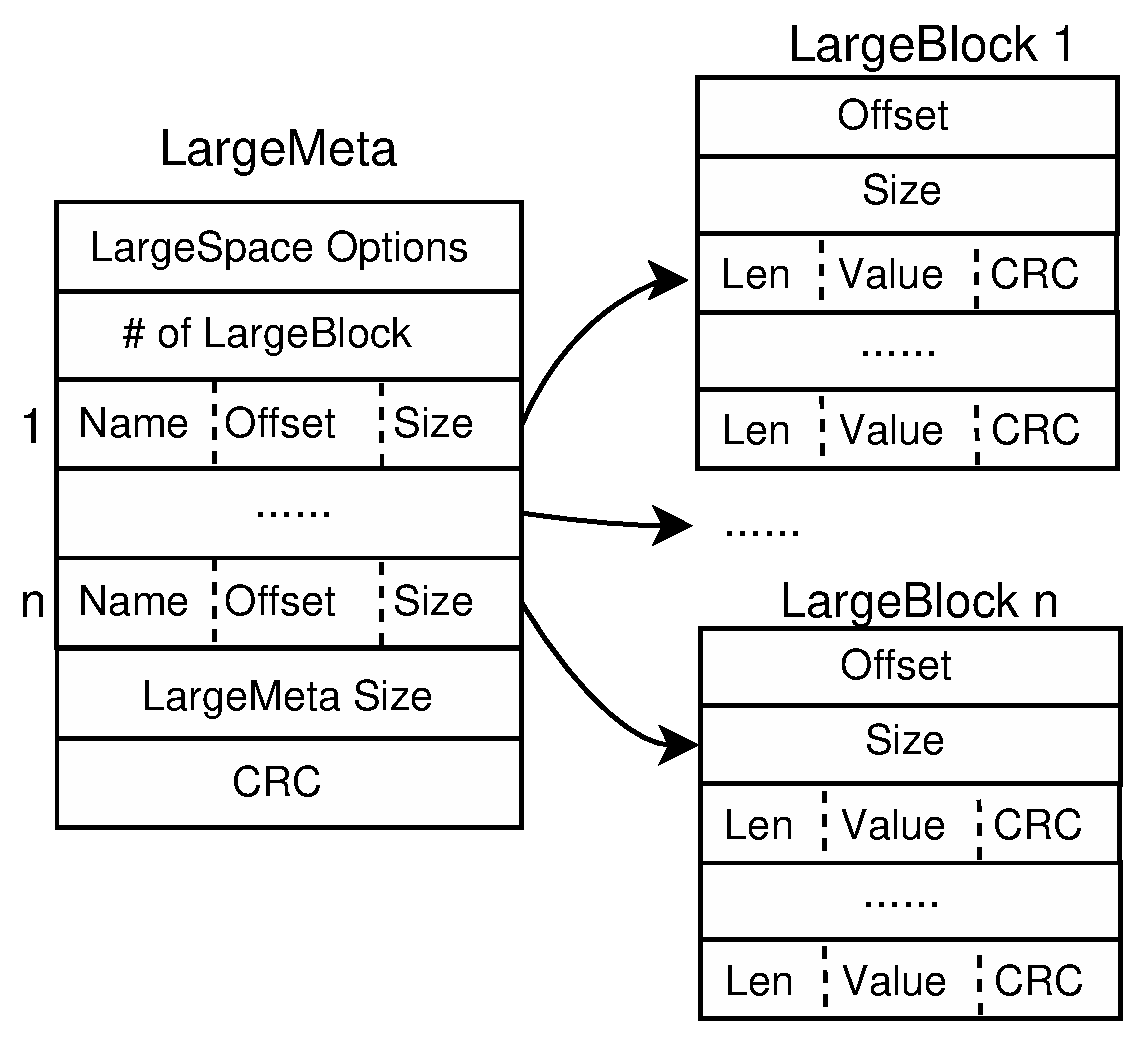
\epsfig{file=figures/large-space.eps,width=.70\linewidth}
\caption{Large Space}
\label{fig:space}
\end{centering}
\end{figure}

Based on the idea of saving different data on different media, we
modify LevelDB to save large values separately into a space called
LargeSpace. LargeSpace is essentially a log and can be saved in media
different from the SSTables. Upon a request of insertion, the value is
appended into LargeSpace and an address is returned. The address is
used for later retrieve of the value. To ease management, LargeSpace
is splited into files called LargeBlocks. The threshold of split,
called SplitThreshold, is a configurable parameter with a default
value of 64MB. Although LargeSpace is split, we enforce that no
value will be splited among LargeBlocks. Therefore, it is possible
that a LargeBlock is larger than the split threshold if there is a
huge value in that LargeBlock.  LargeBlocks are recorded in a metadata
file called LargeMeta. The formats of LargeMeta and LargeBlock and
their relationship is illustrated in Figure~\ref{fig:space}.

It is worth notice that LargeMeta is an immutable file. A new one is
created every time it is updated. LargeMeta can be readily rebuilt
using information from LargeBlocks. Many versions of LargeMeta are
kept which provides a natural support for versioning. This makes the
metadata resistant to hazardous situations such as system crash and
file corruption.

\begin{figure}[t]
\begin{centering}
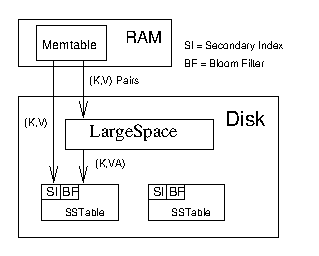
\epsfig{file=figures/mris-store.eps,width=.70\linewidth}
\caption{MRIS Insertion.}
\label{fig:mrisinsert}
\end{centering}
\end{figure}

A large key/value pair will be saved in LargeSpace when its value size
is larger than a configurable threshold, named \texttt{SizeThreshold}.
SizeThreshold provides a simple but effective knob to tradeoff between
cost and performance when LargeSpace and SSTable are stored in
different places. We plan to use more sophisticated algorithm to
determine where to place a certain pair considering not only size but
also hotness and access pattern.

%Insertion of MRIS is illustrated in Figure~\ref{fig:mrisinsert}.
When key/value pairs are firstly inserted into Memtable, they are
treated equally. Large pairs in a Memtable are checked when the
Memtable becomes full and is dumped into SSTable. Whereas small pairs
go to SSTable without touch, the value of large pairs are firstly
inserted into LargeSpace. For each large pair, a new pair is formed
and inserted into SSTable. The key of the new pair is the same as the
old key except its \texttt{KeyType} is changed to indicate that it
represents a large pair.  The value of the new pair contains the size
of the original value, and its addresses in LargeSpace.

%%%%%%%%%%%%%%%%%%%%%%%%%%%%%%%%%%%%%%%%%%%%%%%%%%%%%%%%%%%%%%%%%%%%%%%%%%%%%%
%% For Emacs:
% Local variables:
% fill-column: 70
% End:
%%%%%%%%%%%%%%%%%%%%%%%%%%%%%%%%%%%%%%%%%%%%%%%%%%%%%%%%%%%%%%%%%%%%%%%%%%%%%%
%% For Vim:
% vim:textwidth=70 noai nocin nosi
%%%%%%%%%%%%%%%%%%%%%%%%%%%%%%%%%%%%%%%%%%%%%%%%%%%%%%%%%%%%%%%%%%%%%%%%%%%%%%
% LocalWords:  SSTable LevelDB Memtables
